\documentclass{beamer}
\usepackage{amsmath}
\usepackage{amsfonts}
\usepackage{amssymb}
\usepackage{multicol}
\usepackage{booktabs}
\usepackage{setspace}
\usepackage{bm}
%\usepackage{ctex} 汉语包
\usetheme{Ilmenau}
\usecolortheme{dolphin}

%初始化设置
%配色网站:https://mpetroff.net/files/beamer-theme-matrix/

\title{Bond Risk Premia with Machine Learning}
\author{ZhangMingyue\quad YaoZongqing\quad HeRouhan\quad QuMingqi\\
\quad ZhangYanhui\quad HuangNiyuan\quad ChenYirui\quad LiXinyi}
\institute{ZheJiang University}
\date{\today}

%封面设置

\begin{document}

\frame{\titlepage}

\begin{spacing}{1.2}
    \begin{frame}{Outline}
      \begin{multicols}{2}
      \large{\tableofcontents}
      \end{multicols}
    \end{frame}
\end{spacing}


%目录设置

\section{Introduction}
\frame
{
  \frametitle{Introduction}

  \begin{itemize}
    \item<1-> 
    Our work \textbf{extends Ludvigson and Ng (2009) classic regressions}. We selected forward rates, macroeconomic fundamentals and added factors of investors' subjective beliefs and the supply of government debt to run the regression. 
    \item<2-> 
    We selected the nine most representative macro variables, \textbf{introduced two other dimensional explanatory variables}, conducted regression tests using the data, and found that these factors significantly affect the in-sample excess return fit.
    \item<3->     
    We then used \textbf{a machine learning algorithm} to obtain a model that could predict excess returns better by adjusting the parameters and constructed a simple strategy that, after back-testing, achieved positive excess returns.
  \end{itemize}
}

\section{Literature Review}
\frame{
    \frametitle{Literature Review}

    \begin{itemize}
        \item <1-> 
        Fama and Bliss(1987)
        \tiny
        \begin{equation}
            r(x-1:t+1)-r(x-1:t)=-a_2+(1-b_2)[f(x,x-1:t)-r(1:t)]-u_2(t+1)
        \end{equation}
        
        \item <2-> 
        \normalsize{Cochrane and Piazzesi (2005)}
        \scriptsize
        \begin{equation}
            rx^{(n)}_{t+1}=\beta^{(n)}_{0}+\beta^{(n)}_{1}y^{(1)}_{t}+\beta^{(n)}_{2}f^{(2)}_{t}+\ldots+\beta^{(n)}_{5}f^{(5)}_{t}+\varepsilon^{(n)}_{t+1}
        \end{equation}

        \item <3-> 
        \normalsize{Ludvigson and Ng (2009)}
        \scriptsize
        \begin{equation}
            rx^{(n)}_{t+1}=\beta_{0}+\beta^{'}_{1}\widehat{F_{t}}+\beta_{2}CP_{t}+\varepsilon_{t+1}
        \end{equation}
        
        
    \end{itemize}
}

\frame{
    \frametitle{Literature Review}

    \begin{itemize}
        \item <1-> 
        Laborda and Olmo (2014) incorporate a sentiment factor to document a positive relationship between investor sentiment and expected excess bond returns. 
        \item <2->
        Robin Greenwood and Dimitri Va (2014) proved that the supply and maturity structure of government debt are positively correlated with bond yields and expected returns.
        \item <3->
        Additionally, holding the short rate constant,these effects should be stronger for longer-maturity bonds and during times when arbitrageurs are more risk-averse.
    \end{itemize}
}

\section{Theoretical Framework}
\subsection{Model Theory}
\frame{
    \frametitle{Model Theory}

    \begin{itemize}
        \item <1->
        Our theory mainly builds on the model of Ludvigson and Ng (2009) and Cochrane and Piazzesi (2005).  Variables on the supply of government debt and investor sentiment to optimize were added according to our empirical principles of economics to improve the classical model's predictive ability.
        \item <2->
        We believe that \textbf{the linear combination of forward rates can predict the future inflation rate well.}
    \end{itemize}
}

\frame{
    \frametitle{{Model Theory}}

    \begin{itemize}
        \item <1->
        According to the multi-collinearity between variables and the degree of influence on bond prices, we screen out 9 variables that we believe to be potentially influential factors. 
        \item <2->
        In addition, we choose the variable of exchange rate(Ex rate) to reflect the level of interest rates and CPI as the inflation factor.
        \item <3->
        We also consider the role of sentiment factor and the bond supply with statistical power to explain variation on the bond risk premium.
    \end{itemize}

}

\frame{
    \frametitle{Model Theory}

    \begin{center}
        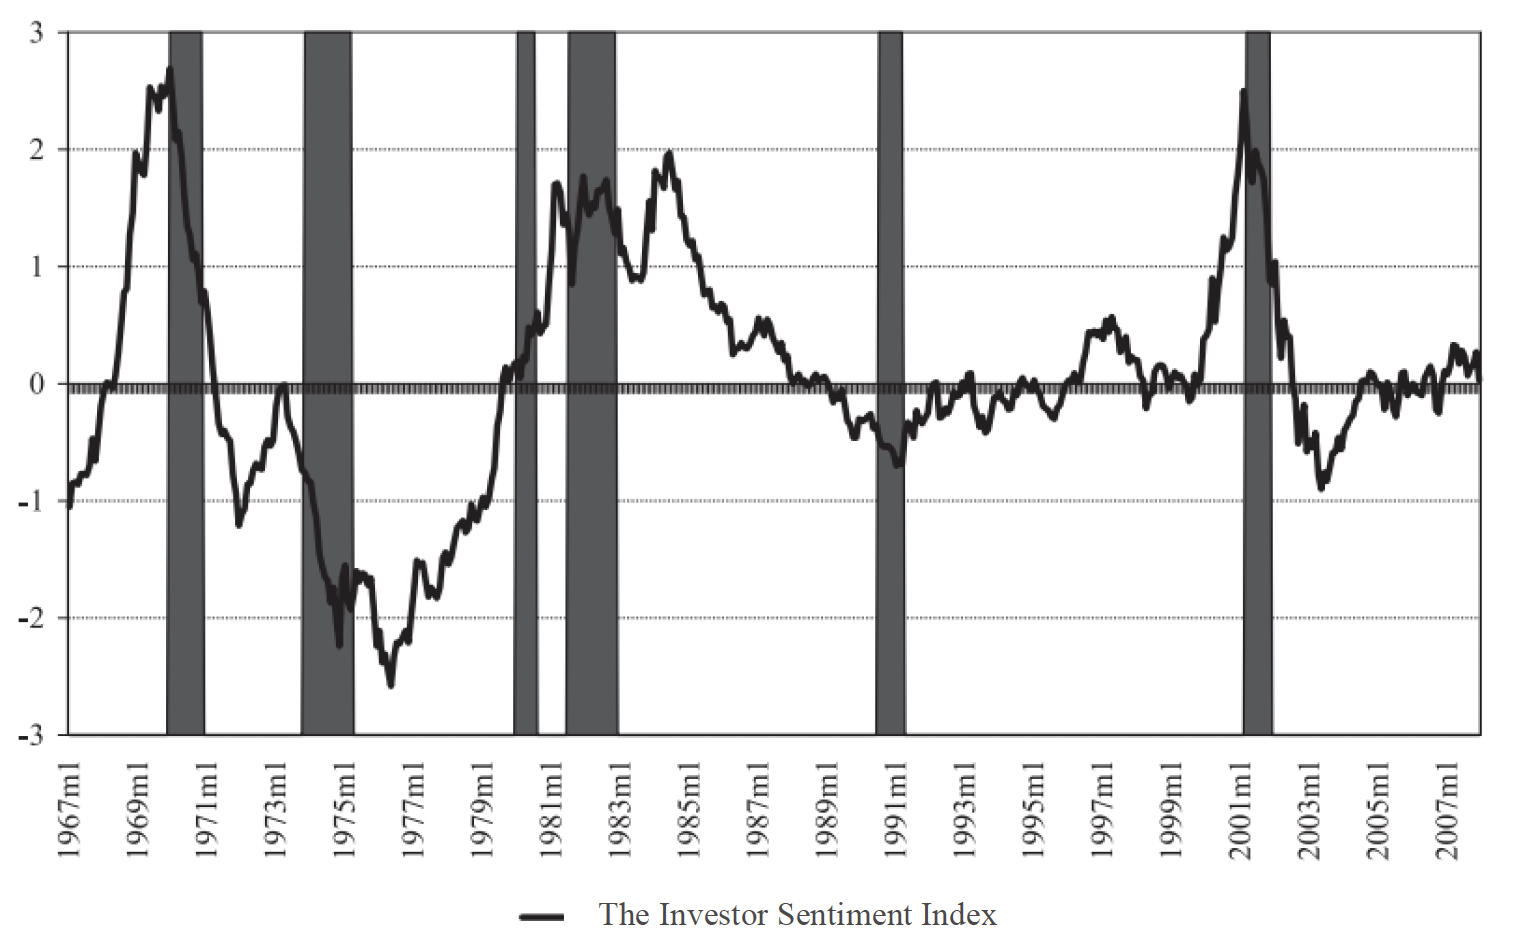
\includegraphics[scale=0.38]{Figure1.png}
    \end{center}
}

\section{Data and Methodology}
\subsection{Definitions of Variables}
\frame{
    \frametitle{Definitions of Variables}

    \begin{center}
        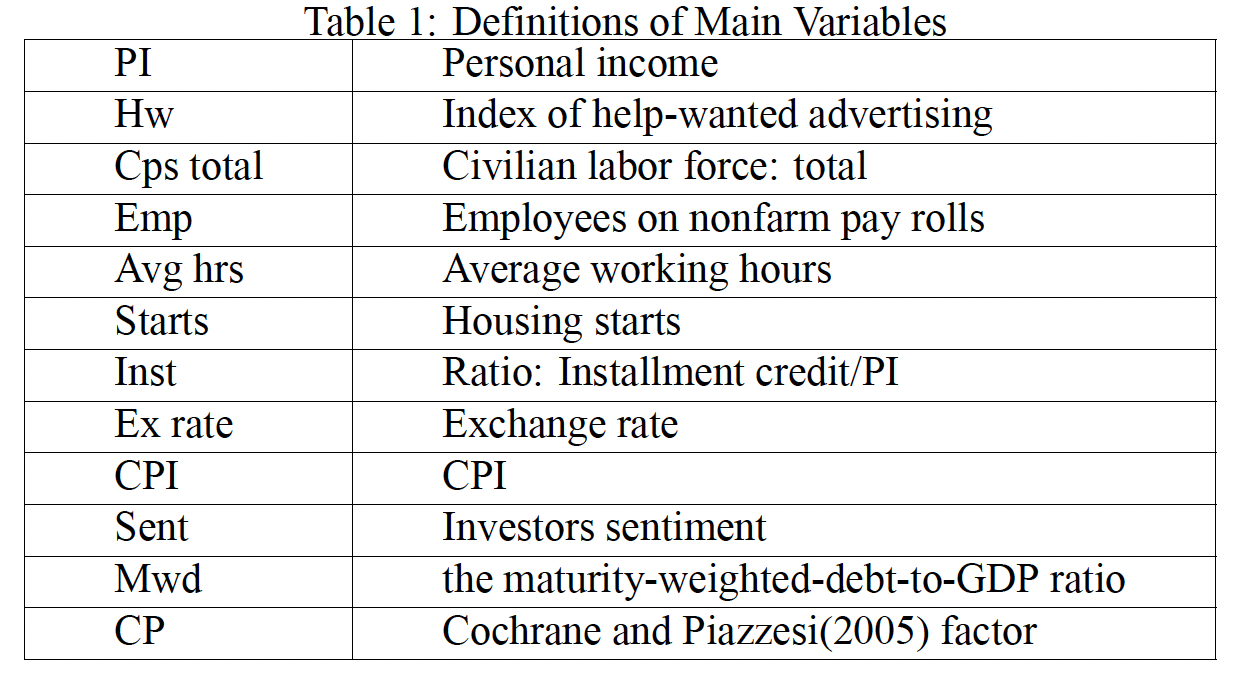
\includegraphics[scale=0.5]{Figure1-Table-1.png}
    \end{center}
}

\subsection{Basic Data}
\frame{
    \frametitle{Basic Data Parameters}

    \begin{center}
        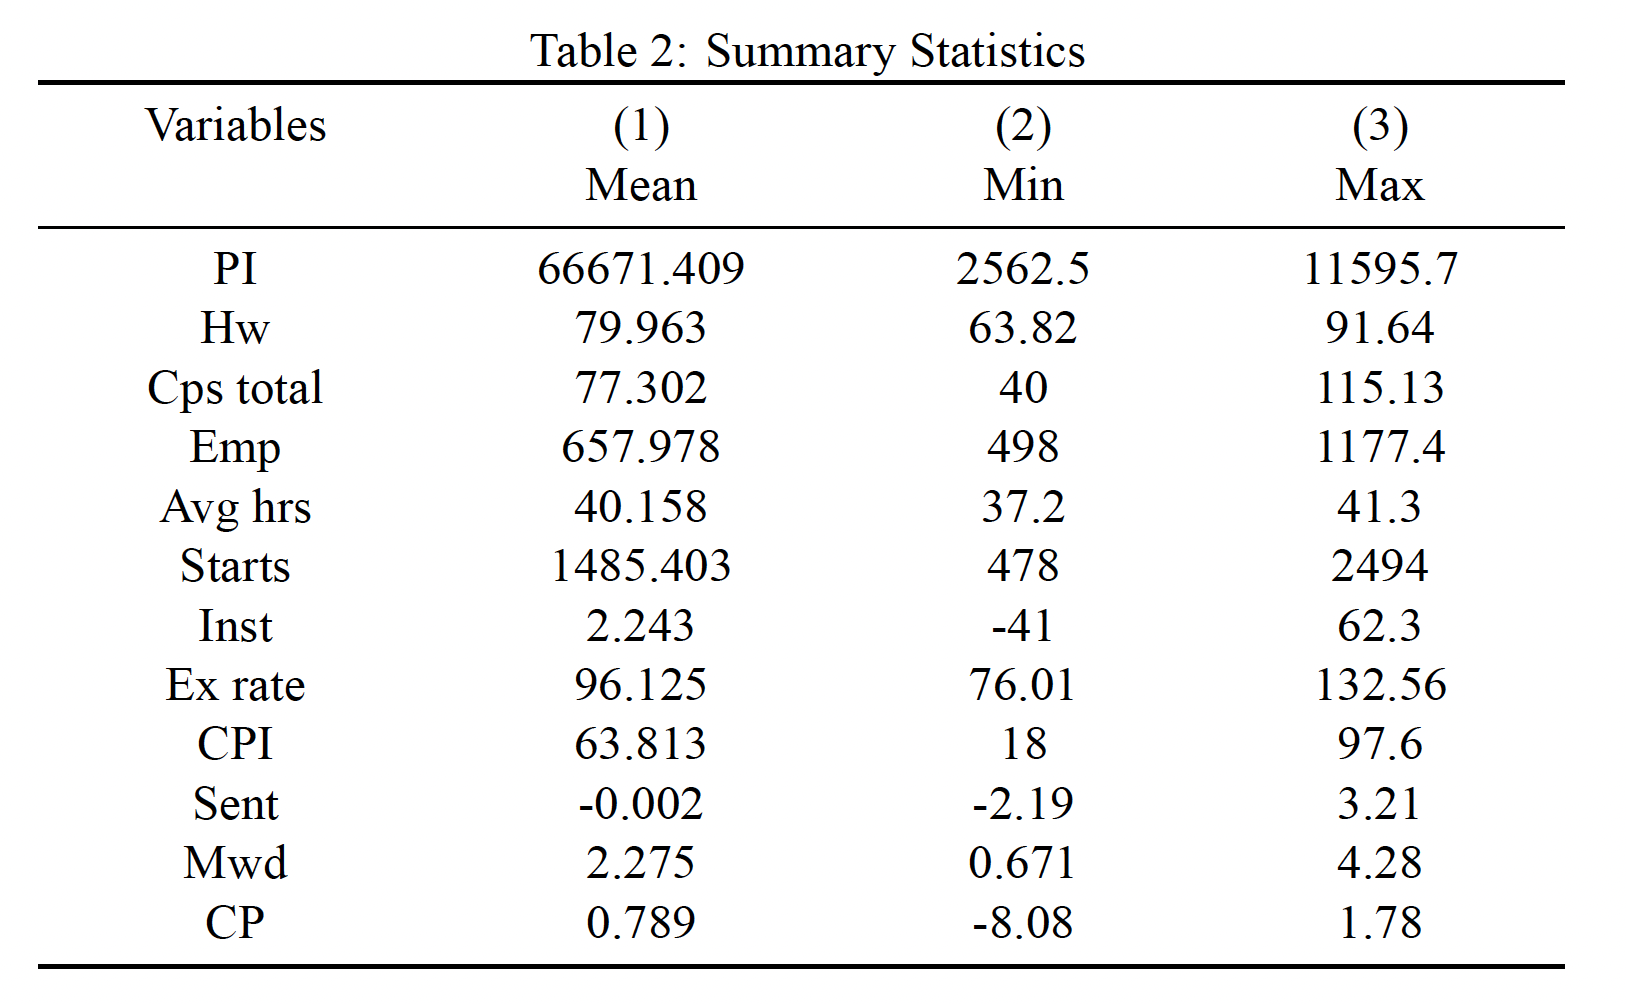
\includegraphics[scale=0.36]{Figure2-Table-2.png}
    \end{center}
}

\frame{
    \frametitle{Empirical Results}

    \begin{center}
        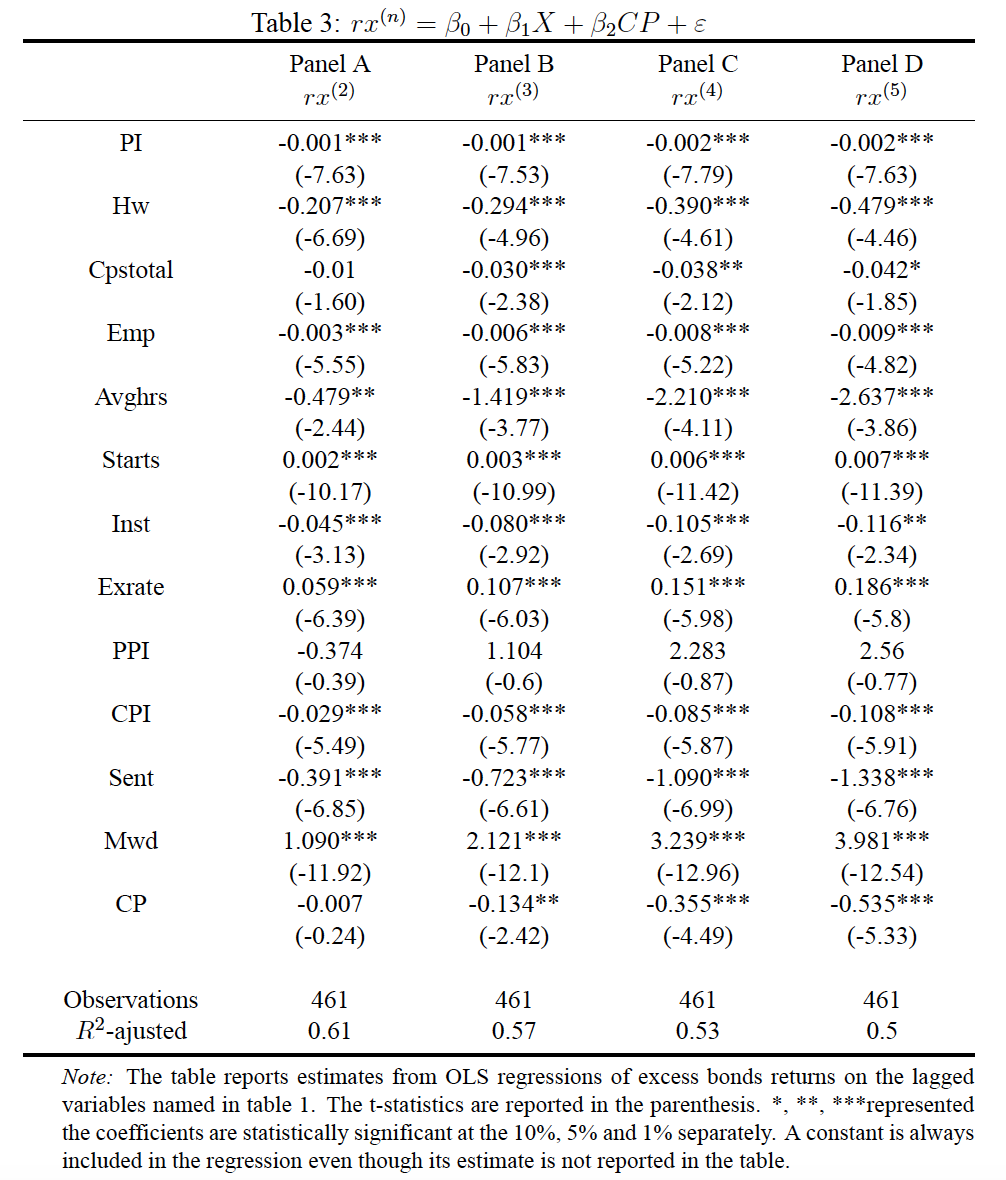
\includegraphics[scale=0.32]{Figure3-Table-3.png}
    \end{center}
}

\subsection{Model Optimization}
\frame{
    \frametitle{Model Optimization}

    \begin{theorem}
        The algorithm is to initialize multiple weak learners and iteratively train them to finally obtain the final learner, thus solving the overfitting problem generated by a single learner fitting too strongly to the sample. 
    \end{theorem}
}

\frame{
    \frametitle{Model Optimization}

    \begin{itemize}
        \item 
        The figure below illustrates a series of training and testing sets, where \textbf{the blue observations constitute the training set and the orange observations constitute the testing set.}
    \end{itemize}
    
    \begin{center}
        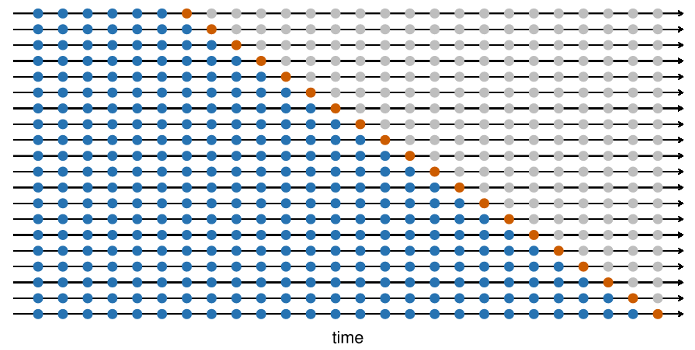
\includegraphics[scale=0.6]{Figure2.png}
    \end{center}
}

\section{Robustness Check}
\subsection{Basic Data}
\frame{
    \frametitle{Robustness Check}

    \begin{itemize}
        \item <1->
        In the multiple linear regression model, the in-sample determinable coefficients are still good, but the out-of-sample determinable coefficients perform poorly.
        \item <2->
        It can also be found that the out-of-sample R-squared is even negative for two-year and three-year bonds, while the out-of-sample prediction improves as maturity rises, which we explain by the fact that the noise cancels each other out as the time period increases.
    \end{itemize}
}

\frame{
    \frametitle{Robustness Check}

    \begin{center}
        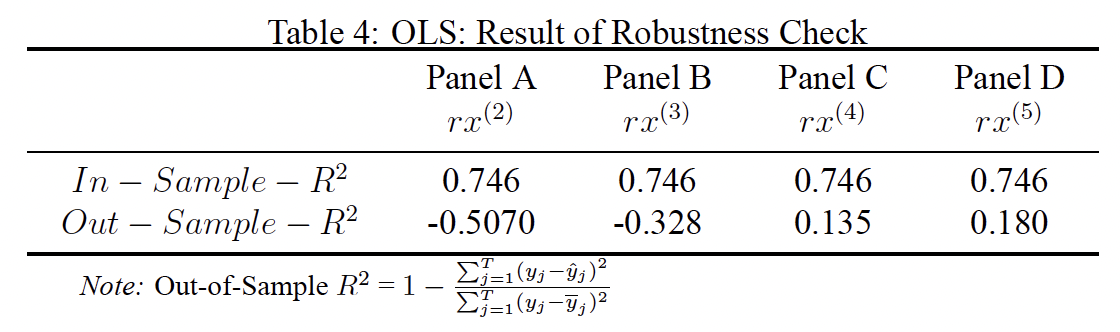
\includegraphics[scale=0.5]{Figure4-Table-4.png}
    \end{center}
}

\frame{
    \frametitle{Robustness Check}

    \begin{center}
        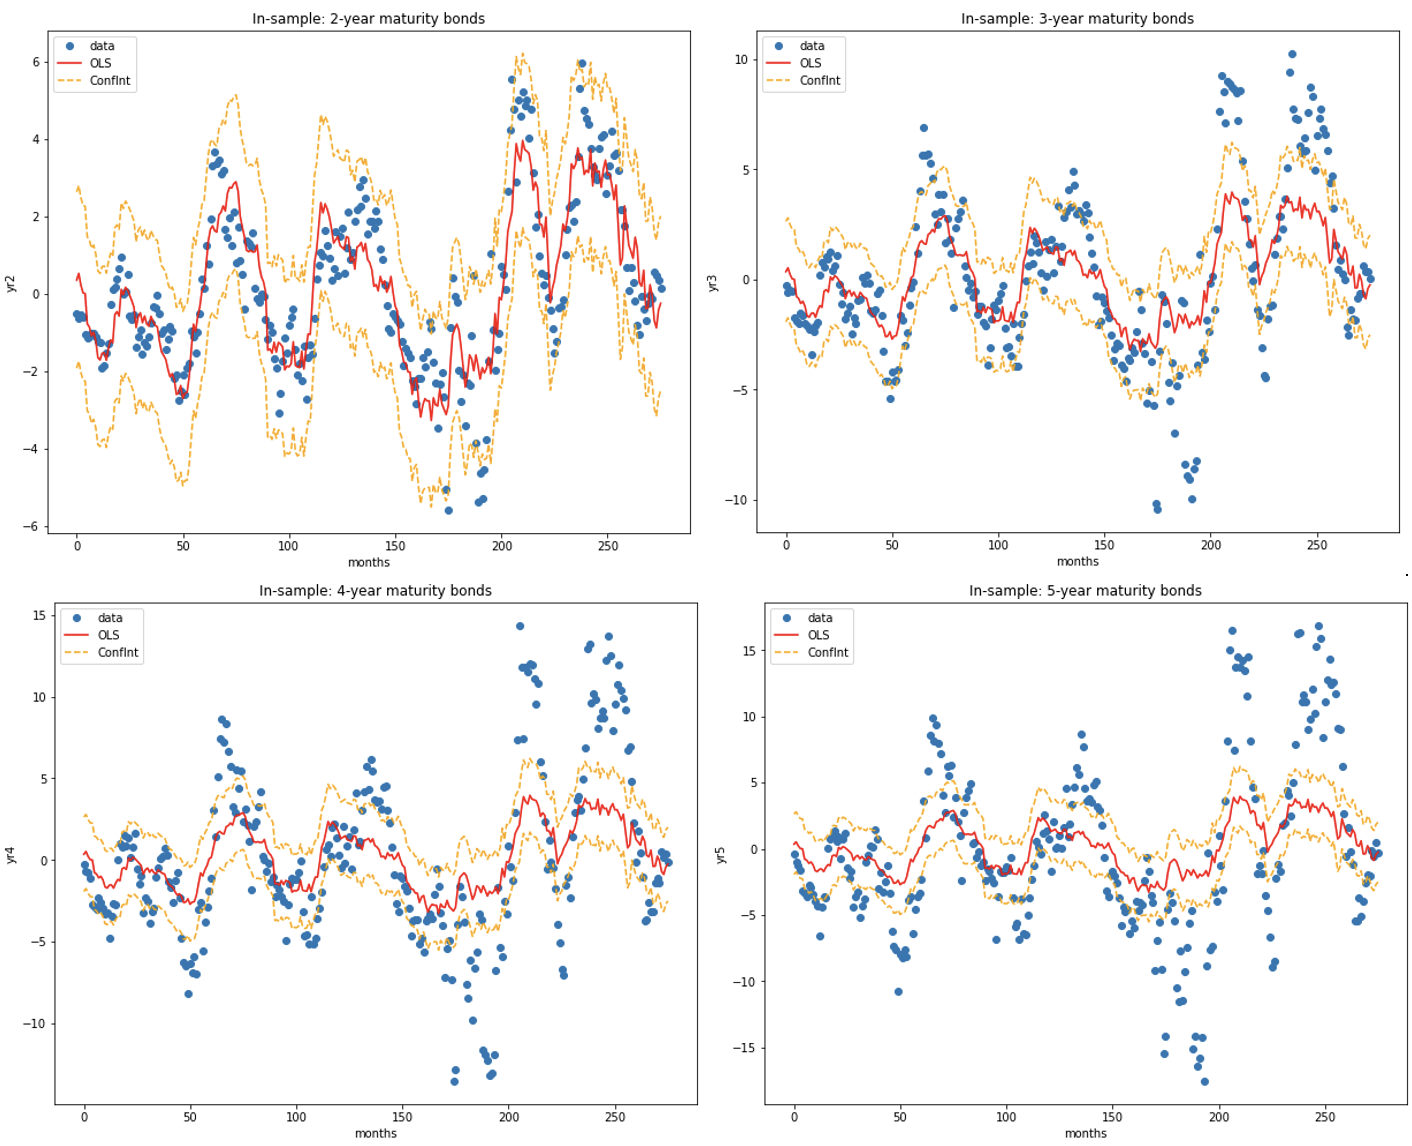
\includegraphics[scale=0.32]{Figure3.png}
    \end{center}
}

\frame{
    \frametitle{Robustness Check}

    \begin{center}
        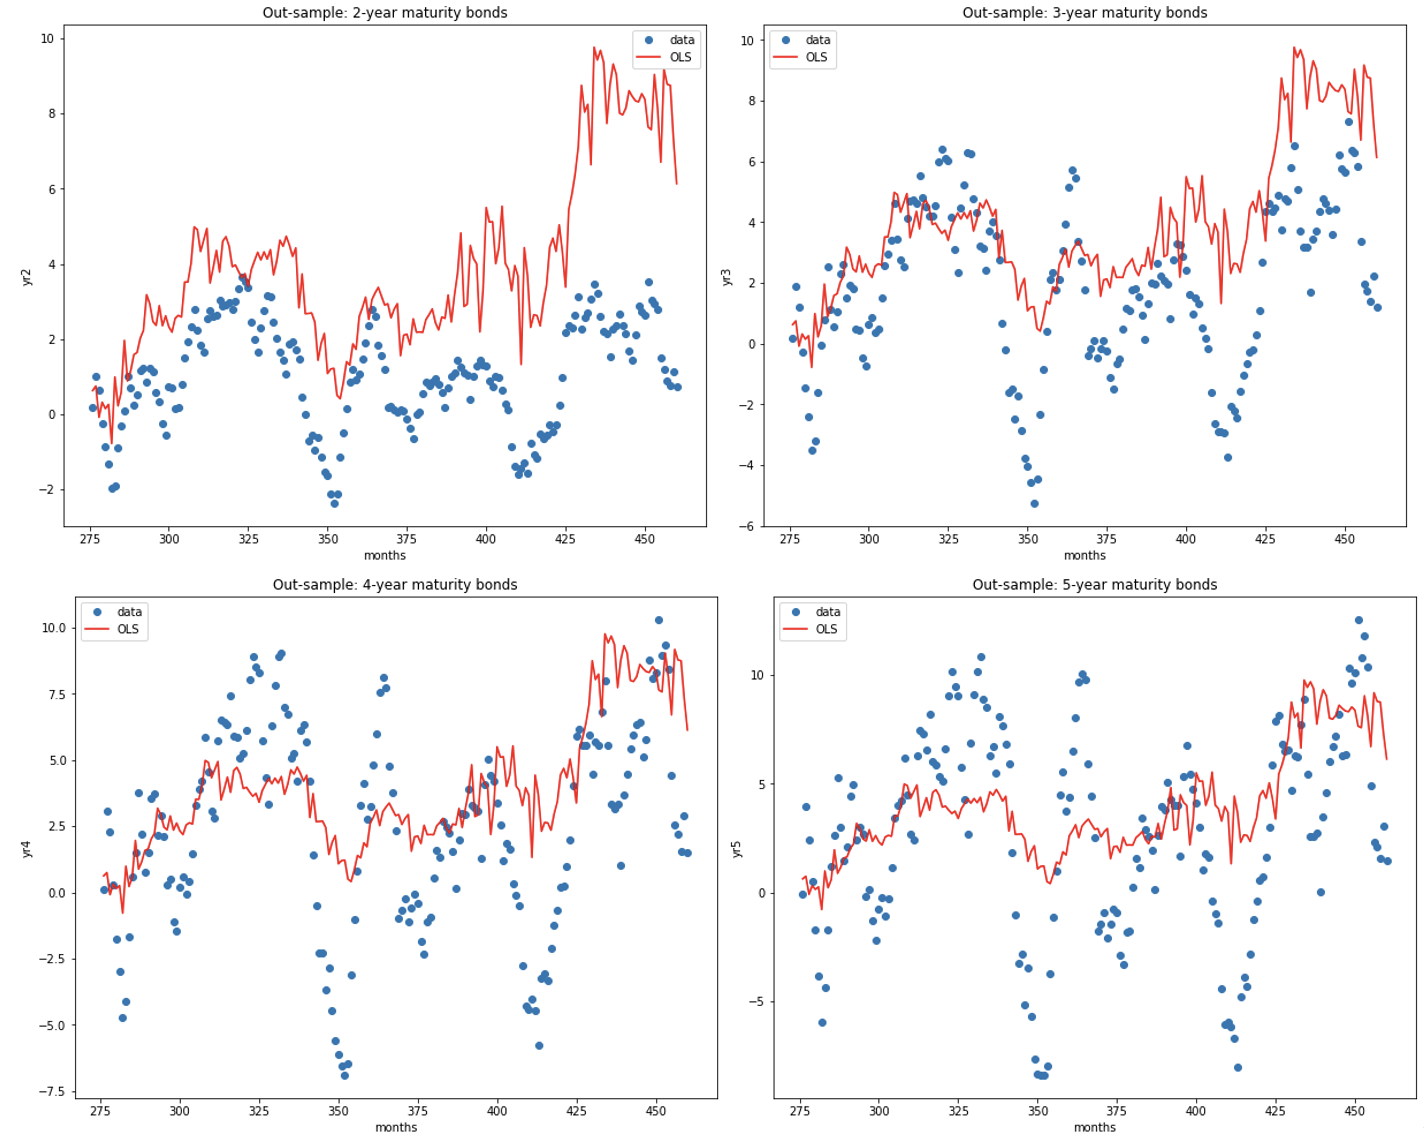
\includegraphics[scale=0.32]{Figure4.png}
    \end{center}
}

\subsection{Model Optimization}
\frame{
    \frametitle{Robustness Check}

    \begin{itemize}
        \item <1->
        As for machine learning, after cross-validation to adjust the hyperparameters and bringing in out-of-sample data regression, the model achieves good explanatory power in the training group, cross-test group and out-of-sample prediction group.
        \item <2->
        Meanwhile, a simple strategy is constructed, i.e., buying bonds when the excess return is predicted to be positive, otherwise no operation is performed, and the yield is simulated in the out-of-sample data, and positive returns are achieved in all four groups of bonds with different maturities.
    \end{itemize}
}

\frame{
    \frametitle{Robustness Check}

    \begin{center}
        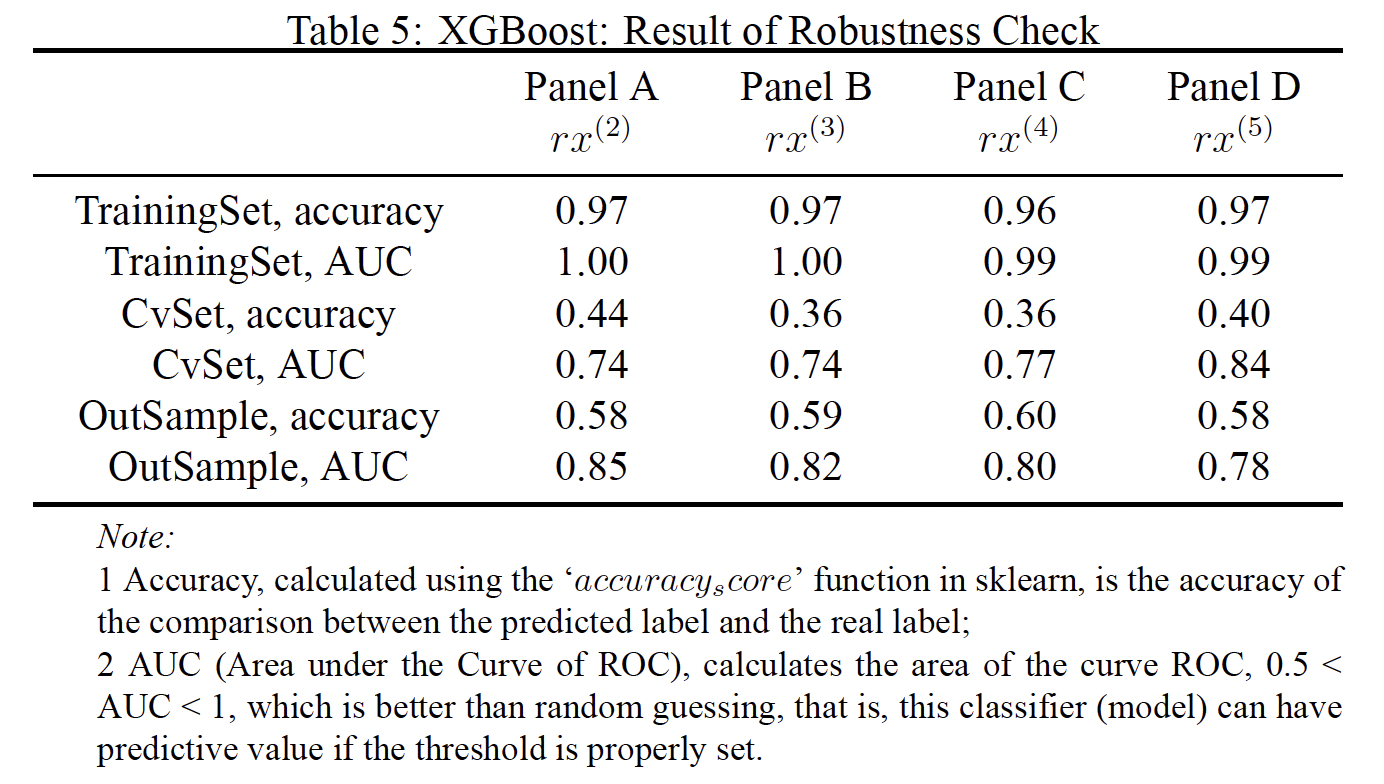
\includegraphics[scale=0.4]{Figure5-Table-5.png}
    \end{center}
}

\frame{
    \frametitle{Robustness Check}

    \begin{center}
        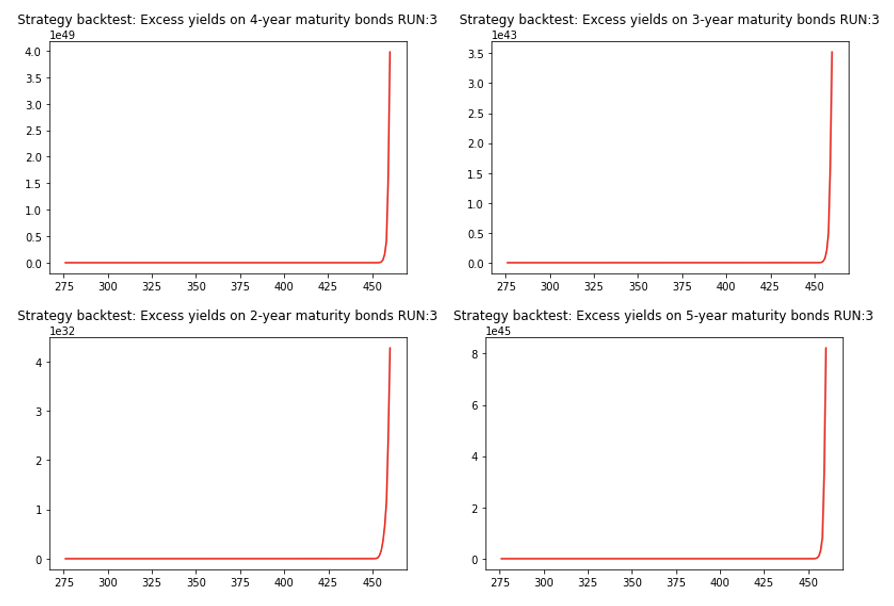
\includegraphics[scale=0.6]{Figure5.png}
    \end{center}
}

\section{Conclusion}
\frame{
    \frametitle{Conclusion}

    \begin{itemize}
        \item <1->
        Our main contribution is the comprehensive analysis through the addition of multiple factors, that is above and beyond the information contained in the term structure of bonds and macroeconomic factors.
        \item <2->
        Also, we back-tested our model with a simple trading strategy and confirmed that it is possible to learn these variables using the XGBoost model to achieve positive returns.
    \end{itemize}
}

\section*{Reference}
\frame
{
    \frametitle{Reference}

    \begin{itemize}
        \item 
        \footnotesize{Sydney C Ludvigson and Serena Ng. Macro factors in bond risk premia. \textit{The Review of Financial Studies}, 22(12):5027–5067, 2009.}
        \item
        \footnotesize{Eugene F Fama and Robert R Bliss. The information in long-maturity forward rates. \textit{The American Economic Review}, pages 680–692, 1987.}
        \item
        \footnotesize{John H Cochrane and Monika Piazzesi. Bond risk premia. \textit{American economic review}, 95(1):138–160, 2005.}
        \item
        \footnotesize{Ricardo Laborda and Jose Olmo. Investor sentiment and bond risk premia. \textit{Journal of Financial Markets}, 18:206–233, 2014.}
        \item
        \footnotesize{Robin Greenwood and Dimitri Vayanos. Bond supply and excess bond returns. \textit{The Review of Financial Studies}, 27(3):663–713, 2014.}
        \item
        \footnotesize{Malcolm Baker and Jeffrey Wurgler. Investor sentiment and the cross-section of stock returns. \textit{The journal of Finance}, 61(4):1645–1680, 2006.}
        \item
        \footnotesize{Tianqi Chen and Carlos Guestrin. Xgboost: A scalable tree boosting system. In \textit{Proceedings of the 22nd acm sigkdd international conference on knowledge discovery and data mining}, pages 785–794, 2016.}
    \end{itemize}
}
\end{document}